\paragraph{QuizziPedia::Front-End::Directives::ExamModalityDirective}
\begin{figure} [ht]
	\centering
	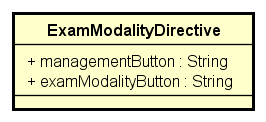
\includegraphics[scale=0.80]{UML/Classi/Front-End/QuizziPedia_Front-end_ExamModalityDirective.png}
	\caption{QuizziPedia::Front-End::Views:ExamModalityDirective}
\end{figure} \FloatBarrier
\begin{itemize}
	\item \textbf{Descrizione}: directive contenete i componenti grafici per attivare la modalità esame su un questionario e gestire le iscrizioni;
	\item \textbf{Utilizzo}: permette di attivare la modalità esame su un questionario e di gestirne le iscrizioni;
	\item \textbf{Relazioni con altre classi}:
	\begin{itemize}
		\item \textit{IN} \texttt{QuizEventController}: questa classe permette di reagire ai comandi dell'utente durante la gestione dei suoi questionari;
		\item \textit{IN} \texttt{QuizEventModelView}: classe di tipo modelview la cui istanzazione è contenuta all'interno della variabile di ambiente \$scope di \texttt{Angular.js}. All'interno di essa sono presenti le variabili e i metodi necessari per il \textit{Two-Way Data-Binding\ped{G}} tra la view \texttt{QuizEventView} e il controller \texttt{QuizEventController};
		\item \textit{IN} \texttt{QuestionnaireManagementView}: view principale per la gestione dei questionari; 
		\item \textit{IN} \texttt{LangModel}: rappresenta il modello delle informazioni per la giusta traduzione dell'applicazione.
	\end{itemize}
		\item \textbf{Attributi}:
		\begin{itemize}
			\item {+ managementButton: String} \\ Attributo che viene utilizzato per visualizzare la giusta traduzione della \textit{label\ped{G}} per il bottone di gestione delle iscrizioni al questionario selezionato, in italiano o in inglese; 
			\item {+ examModalityButton: String} \\ Attributo che viene utilizzato per visualizzare la giusta traduzione della \textit{label\ped{G}} per il bottone di attivazione della modalità esame del questionario selezionato, in italiano o in inglese;
			\item \texttt{+ controller: String} \\ Stringa contenente il nome del controller della direttiva;
			\item \texttt{+ restrict: String} \\ Stringa che permette di definire le modalità di inserimento della direttiva all'interno della pagina;
			\item \texttt{+ scope: Scope} \\ Oggetto scope interno della direttiva, contiene le funzionalità per gestire i dati presenti all'interno;
			\item \texttt{+ templateUrl: String} \\ Stringa contenente il percorso del file \textit{HTML\ped{G}} che contiene la direttive.
		\end{itemize}
\end{itemize}